\documentclass[conference]{IEEEtran}
\IEEEoverridecommandlockouts
\usepackage{cite}
\usepackage{amsmath,amssymb,amsfonts}
\usepackage{algorithm}
\usepackage{algorithmic}
\usepackage{graphicx}
\usepackage{textcomp}
\usepackage{xcolor}
\usepackage{enumerate}
\usepackage{multirow}
\def\BibTeX{{\rm B\kern-.05em{\sc i\kern-.025em b}\kern-.08em
    T\kern-.1667em\lower.7ex\hbox{E}\kern-.125emX}}


\newcommand{\rmnum}[1]{\expandafter{\romannumeral #1\relax}}
\begin{document}

\title{Adaptive Metamorphic Testing\\
\thanks{}
}

\author{
\IEEEauthorblockN{1\textsuperscript{st} Chang-ai~Sun, Hepeng Dai}
\IEEEauthorblockA{\textit{School of Computer and Communication Engineering} \\
\textit{University of Science and Technology Beijing}\\
Beijing, China \\
casun@ustb.edu.cn, daihepeng@xs.ustb.edu.cn}
\and
\IEEEauthorblockN{2\textsuperscript{rd} Tsong Yueh~Chen}
\IEEEauthorblockA{\textit{Faculty of Information and Communication Technologies} \\
\textit{Swinburne University of Technology Australia}\\
Melbourne, Australia \\
tychen@swin.edu.au}
}

\maketitle

\begin{abstract}
  Metamorphic testing (MT) is a promising technique to alleviate the oracle problem, which first defines metamorphic relations (MRs) to generate new test cases (i.e. follow-up
  test cases) from the original test cases (i.e. source test cases), then the results of source and follow-up test cases are verified against the relevant MRs.
  To improve the effectiveness of MT, researchers have focused their effort on generating better MRs or source test cases, while ignoring the impact of test execution.
  Most of traditional MT techniques employ random testing strategy (RT) to select source test cases. It may not be efficient because RT does not use any information of the software under test.
  This study aims to improve the efficiency of MT through controlling the execution process of MT, and proposes a adaptive metamorphic
  testing (AMT) technique. We conduct a empirical study where AMT is employed to test three real-life programs. The results of empirical study show that AMT outperforms traditional
  MT in terms of fault-detecting efficiency.
\end{abstract}

\begin{IEEEkeywords}
metamorphic testing, control test process, random testing
\end{IEEEkeywords}

\section{Introduction}
\label{section:introduction}
Test result verification is an important part of software testing. A test oracle \cite{weyuker1982testing} is a mechanism that can exactly decide whether the output
produced by a programs is correct. However, there are situations where it is difficult to decide whether the result of the software under test (SUT) agrees with the expected
result. This situation is known as oracle problem \cite{barr2015oracle, patel2018mapping}. In order to alleviate the oracle problem, several techniques have been proposed such as
N-version testing \cite{brilliant1990performance}, metamorphic testing (MT) \cite{chen1998metamorphic, chen2018metamorphic}, assertions \cite{sim2014eliminating}, machine
learning \cite{chan2009pat}, etc. Among of them, MT obtains metamorphic relations (MRs) according to the properties of SUT. Then, MRs are used to generate new test cases called
follow-up test cases from original test cases known as source test cases. Next, both source and follow-up test cases are executed and their result are verified against the corresponding
MRs.

The fault-detecting effectiveness of MT relies on the quality of MRs and the source test cases. There are astronomically large number of studies to investigate generate
good MRs \cite{chen2004case, cao2013correlation, sun2011metamorphic, chen2014metric, xie2016looking} or the source test cases \cite{chen2004metamorphic,
batra2011efficient,
dong2013security}. However, Researchers ignore the
impact of test execution on the efficiency of MT. Random testing (RT) that randomly selects test cases from input domain (which refers to the set of all possible inputs of SUT), which
is most
commonly used technique in traditional MT \cite{segura2016survey}. Although RT is simple to implement, RT does not make use of any execution information about SUT or the test history.
Thus,
traditional MT may be inefficient in some situations.

In contrast to RT, partition testing (PT) attempts to generate test cases in a more systematic way, aiming to use fewer test cases to detect more faults. When conducting
PT, the input domain of SUT is divided into disjoint partitions, with test cases then selected from each and every one. Each partition is expected to have a certain degree
of homogeneity, that is, test cases in the same partition should have similar software execution behavior: If one input can detect a fault, then all other inputs in the same partition
should also be able to detect a fault.
RT and PT have their own characteristics. Therefore, it is a nature thought to investigate the integration of them for developing new testing techniques.
Sun et al. \cite{sun2018adaptive} proposed adaptive partition testing (APT) that takes advantages of testing information to control the testing process, with the goal of benefitting
from
the advantages of RT and PT.

In this study, we investigate how to make use of feedback information in the previous tests to control the execution process of MT, and propose a adaptive metamorphic testing framework
based on PT to
improve the fault-detecting efficiency of MT. We conduct an empirical study to evaluate proposed technique. The paper makes the following contributions:

\begin{enumerate}[(1)]
  \item
  An adaptive metamorphic testing framework is proposed, which combines the basic principle of MT and software cybernetics \cite{cai2002optimal}.
  \item
  An MRs-centric adaptive metamorphic testing technique (M-AMT) which used a feedback mechanism to control the execution process of MT.
  \item
  An empirical study has been conducted to evaluate the fault detection efficiency of the proposed AMT, where three Java programs are selected as subjects to
  compare the performance of traditional MT and AMT in terms of fault detection efficiency and time overhead.
\end{enumerate}

The rest of the paper is organized as follows. Section \ref{section:background} introduces the underlying concepts related to MT and DRT.
Section \ref{section:amt} presents the motivation of this study, the framework and algorithms of AMT. Section \ref{section:empirical} describes an empirical study where the proposed
AMT is used to test three real-life programs. The related work is reviewed in Section \ref{section:related}.
Finally, we summarize our work in Section \ref{section:conclusion}.


\section{Background}
In this section, we present the basics to understand our approach. we start with a brief introduction to metamorphic testing, and then describe dynamic random testing.
\label{section:background}
\subsection{Metamorphic Testing}
\label{section:mt}
MT is a novel technique to alleviate the oracle problem: Instead of applying an oracle, MT uses a set of MRs (corresponding to some specific properties of the SUT) to verify the
test results. MT is normally conducted according to the following steps:
\begin{description}
  \item [Step1.]
  Identify an MR from the specification of the SUT.
  \item [Step2.]
  Generate the source test case $stc$ using the traditional test cases generation techniques.
  \item [Step3.]
  Derive the follow-up test case $ftc$ from the $stc$ based on the MR.
  \item [Step3.]
  execute $stc$ and $ftc$ and get their outputs $O_s$ and $O_f$.
  \item [Step4.]
  Verify $stc$, $ftc$, $O_s$, and $O_f$ against the MR: If the MR does not hold, a fault is said to be detected.
\end{description}
The above steps can be repeated for a set of MRs.

Let us use a simple example to illustrate how MT works. For instance, consider the mathematic function $f(x,y)$ that can calculate the maximal value of two integers $x$ and $y$.
There is a simple yet obvious property: the order of two parameters $x$ and $y$ does not affect the output, which can be described as the follow metamorphic relation
(MR): $f(x,y) = f(y,x)$. In this MR, $(x,y)$ is source test case, and $(y,x)$ is considered as follow-up test case. Suppose \texttt{P} denotes a program that implements the
function $f(x,y)$, \texttt{P} is executed with a test cases $(1,2)$ and $(2,1)$. Then we check $P(1,2) = P(2,1)$: If the equality does not hold, then we consider that \texttt{P} at
least has one fault.

\subsection{Dynamic Random Testing}
\label{section:drt}
Cai et al \cite{cai2009random} proposed dynamic random testing (DRT), which adjusts the test profile according to the result of current test. In DRT, the input domain is first divided
into $m$ partitions (denoted $s_1, s_2, \ldots, s_m$), and each $s_i$ is assigned a probability $p_i$. During the test process, the selection probabilities of partitions are dynamically
updated. Suppose that a test case $tc$ from $s_i$ ($i = 1,2,\ldots,m$) is selected and executed. The process of DRT adjusting the value of $p_i$ is as follows: If $tc$ detects a fault,
$\forall j = 1, 2, \ldots, m$ and $j \neq i$, we then set

\begin{equation}
\label{eq:DRThitJ}
%\text{new} p_j =
p'_j =
\begin{cases}
p_j - \displaystyle\frac{\epsilon}{m-1} & \text{if } p_j \geq \displaystyle\frac{\epsilon}{m-1} \\
0 & \text{if } p_j < \displaystyle\frac{\epsilon}{m-1}
\end{cases},
\end{equation}
where $\epsilon$ is a probability adjusting factor, and then

\begin{equation}
\label{eq:DRThitI}
  p'_i = 1 - \sum_{\substack{j = 1 \\ j \neq i}}^m p'_j.
\end{equation}

Alternatively, if $tc$ does not detect a fault, we set

\begin{equation}
\label{eq:DRTmissI}
%\text{new } p_i =
p'_i =
\begin{cases}
p_i - \epsilon & \text{if } p_i \geq \epsilon \\
0 & \text{if } p_i < \epsilon
\end{cases},
\end{equation}
and then for $\forall j = 1, 2, \ldots, m$ and $j \neq i$, we set

\begin{equation}
\label{eq:DRTmissJ}
p'_j =
\begin{cases}
p_j + \displaystyle\frac{\epsilon}{m-1} & \text{if } p_i \geq \epsilon \\
p_j + \displaystyle\frac{p'_i}{m-1} & \text{if } p_i < \epsilon
\end{cases}.
\end{equation}

 The detailed DRT algorithm is given in Algorithm \ref{alg:drt}. In DRT, a test case is selected from a partition that has been randomly selected according to the test profile
 $\{\left \langle s_1, p_1 \right \rangle, \left \langle s_2, p_2 \right \rangle, \ldots, \left \langle s_m, p_m \right \rangle\}$ (Lines 2 to 4). If a fault is detected, then
 Formulas \ref{eq:DRThitJ} and \ref{eq:DRThitI} are used to adjust the values of $p_i$ (Line 6), otherwise Formulas \ref{eq:DRTmissI} and \ref{eq:DRTmissJ} are used (Line 8).
 This process is repeated until a termination condition is satisfied (Line 1). Examples of termination conditions can be ``when the testing resources are exhausted,'' ``when a
 certain number of test cases have been executed,'' ``when the first faults is detected,'' etc.

 In AMT, When a source test case and corresponding follow-up test case belong to same partition $s_i$, DRT is employed to update the test profile: If a fault is detected (i.e.,
 their results violate the related MR), then Formulas \ref{eq:DRThitJ} and \ref{eq:DRThitI} are used to adjust the values of $p_i$, otherwise Formulas \ref{eq:DRTmissI}
 and \ref{eq:DRTmissJ} are used. During the testing process, there is the other situation where a source test case and corresponding follow-up test case do not belong to same partition.
 In order to adjust the test profile in this situation, we proposed a new strategy that is described in Section \ref{section:mdrt}.


\begin{algorithm}
\caption{DRT}
\label{alg:drt}
    \begin{algorithmic}[1]
    \renewcommand{\algorithmicrequire}{\textbf{Input:}}
    \renewcommand{\algorithmicendwhile}{\algorithmicend\_\algorithmicwhile}
    \renewcommand{\algorithmicendif}{\algorithmicend\_\algorithmicif}
    \REQUIRE $\epsilon, p_1, p_2, \ldots, p_m$
    \WHILE {termination condition is not satisfied}
    \STATE Select a partition $s_i$ according to the test profile $\{\left \langle s_1, p_1 \right \rangle, \left \langle s_2, p_2 \right \rangle, \ldots, \left \langle s_m, p_m \right
    \rangle\}$.
    \STATE Select a test case $tc$ from $s_i$.
    \STATE Test SUT using $tc$.
    \IF {a fault is detected by $tc$}
    \STATE Update test profile according to Formulas \ref{eq:DRThitJ} and \ref{eq:DRThitI}.
    \ELSE
    \STATE Update test profile according to Formulas \ref{eq:DRTmissI} and \ref{eq:DRTmissJ}.
    \ENDIF
    \ENDWHILE
    \end{algorithmic}
\end{algorithm}

\section{Adaptive Metamorphic Testing}
\label{section:amt}
In this section, we first describe the motivation, then present a framework for improving the efficiency of MT, and finally present an algorithm for AMT, namely MRs-centric adaptive
metamorphic testing (M-AMT).

\subsection{Motivation}
\label{section:motivation}
Since MT was first published, a considerable number of studies have been reported from various aspects \cite{segura2016survey}. To improve the effectiveness of MT, most of studies
have paid their
attention to identify the better MRs, which are more likely to be violated. For the effectiveness of MRs, several factors such as the difference between the source and follow-up
test cases \cite{chen2004case, cao2013correlation} and the the detecting-faults capacity of MRs compared to existing test oracles \cite{liu2014effectively}, have been investigated.

Since the follow-up test cases are generated based on source test cases and MRs, in addition to the so-called good MRs, source test cases also have an impact on the efficiency of MT.
However, 57\% of existing studies employed RT to select test cases, and 34\% of existing studies used existing test suites according to a survey report by Segura et al. in their Journal
\cite{segura2016survey}. In this study, we investigate the strategies of selection test cases and MRs, and its impacts on the fault-detecting efficiency of MT.

It has been pointed out that fault-detecting inputs tend to cluster into ``continuous regions'' \cite{ammann1988data, finelli1991nasa}, that is, the test cases in some partitions are more
likely to detect faults than the test cases in other partitions. Inspired by the observation, AMT takes full advantage of feedback information to update the test profile, aiming at
increasing the selection probabilities of partitions with larger failure rates. Accordingly, the MRs whose sources test cases belonging to the partitions with larger failure rates,
are more likely to be selected and violated. Therefore, AMT is expected to detect faults more efficient than traditional MT.



\subsection{Framework}
\label{section:framework}
To show the idea of controlling the execution precess of MT, we propose a AMT framework illustrated in Figure \ref{fig:framework}, which combines RT and PT to benefit from the advantages
of both. During the testing, the framework make use of feedback information to update the test profile, and a new source test case is selected from a partition that was randomly selected
according to the updated test profile. Meanwhile, an MR is randomly selected from the set of MRs whose source test cases belong to selected partition. We next discuss the individual
framework components.

\begin{enumerate}[(1)]
  \item
  \emph{Partition Construction}
  is responsible to construct partitions. There are a class of testing techniques that break the input domain into a number of partitions \cite{weyuker1991analyzing}. Various approaches
  and principles for achieving convenient and effective partitions have been discussed in the literature \cite{weyuker1991analyzing, cai2005partition, chen1994relationship, chen1996expected}.
  The input domain of the SUT can be partitioned based on the SUT specifications. Once partitioned, testers can assign probability distributions to the partitions as an initial test
  profile. This initial test profile can be assigned in different ways, including using a uniform probability distribution, or one that sets probabilities according to the importance
  of the partition. For instance, a partition should be given a higher priority if more faults have been detected within it in the previous testing history.
  \item
  \emph{Partition Selection}
  randomly selects a partition according to the test profile.
  \item
  \emph{MR and Source Test Case Selection}
  selects an metamorphic relation $MR_i$ based on some strategies from the set of MRs whose source test cases belong to selected partition,
  then randomly select a source test case $stc$ from the selected partition.
  \item
  \emph{Follow-up Test Case Generation}
  derives the follow-up test cases $ftc$ by transforming the source test case $stc$ according to the $MR_i$.
  \item
  \emph{Test Case Execution}
  executes SUT with source and follow-up test cases, and intercepts their results.
  \item
  \emph{Test Profile Adjustment}
  collects the pass and fail status that is determined by verifying the results of source and follow-up test cases against the corresponding MR, and updates the test profile.
  The details of strategies updating test profile are described in Section \ref{section:drt} and \ref{section:mdrt}.
\end{enumerate}


\begin{figure}[htb]
  \centering
  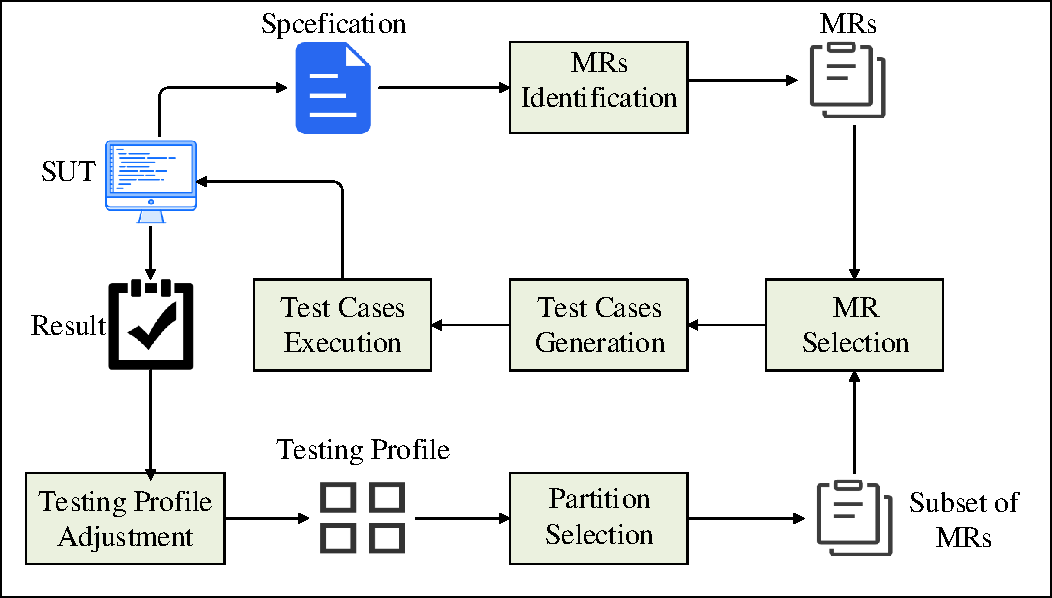
\includegraphics[width = 0.47\textwidth]{figs//framework//framework}
  \caption{The framework of adaptive metamorphic testing}
  \label{fig:framework}
\end{figure}



\subsection{Metamorphic Dynamic Random Testing}
\label{section:mdrt}

When the source test case $stc$ and follow-up test case $ftc$ related to an metamorphic relation $MR$ belong to the same partition $s_i$, DRT is suitable to adjust the test profile.
However, during the test process, there are some scenarios where the $stc$ is not in the same partition as $ftc$. In such scenarios, DRT cannot be used to adjust the test profile.
To solve this problem, we proposed metamorphic dynamic random testing (MDRT).

Suppose that source test case $stc$ and follow-up test case $ftc$ related to an metamorphic relation $MR$, belong to $s_i$ and $s_f$ ($f \in \{1, 2, \ldots, m\}, f \ne i$), respectively.
 If their results violate the $MR$, $\forall j = 1, 2, \ldots, m$ and $j \ne i, f$, we set

\begin{equation}
\label{eq:MDRThitJ}
p'_j =
\begin{cases}
p_j - \displaystyle\frac{2\epsilon}{m-2} & \text{if } p_j \geq \displaystyle\frac{2\epsilon}{m-2} \\
0 & \text{if } p_j < \displaystyle\frac{2\epsilon}{m-2}
\end{cases},
\end{equation}
where $\epsilon$ is a probability adjusting factor, and then

\begin{equation}
\label{eq:MDRThitI}
  p'_i = p_i + \displaystyle\frac{(1-\sum_{\substack{j = 1, j \ne i,m}}^m p_j^{'}) - p_i - p_f}{2},
\end{equation}

\begin{equation}
\label{eq:MDRThitF}
  p'_f = p_f + \displaystyle\frac{(1-\sum_{\substack{j = 1, j \ne i,m}}^m p_j^{'}) - p_i - p_f}{2}.
\end{equation}

Alternatively, if their results hold the $MR_h$, we set

\begin{equation}
\label{eq:MDRTmissI}
p'_i =
\begin{cases}
p_i - \epsilon & \text{if } p_i \geq \epsilon \\
0 & \text{if } p_i < \epsilon
\end{cases},
\end{equation}

\begin{equation}
\label{eq:MDRTmissF}
p'_f =
\begin{cases}
p_f - \epsilon & \text{if } p_f \geq \epsilon \\
0 & \text{if } p_f < \epsilon
\end{cases},
\end{equation}
and then for $\forall j = 1, 2, \ldots, m$ and $j \neq i, f$, we set

\begin{equation}
\label{eq:MDRTmissJ}
p'_j = p_j + \displaystyle\frac{(p_i - p_i^{'}) + (p_f - p_f^{'})}{m - 2}
\end{equation}

The detailed MDRT algorithm is given in Algorithm \ref{alg:mdrt}. In MDRT, the source test case is selected from a partition that has been randomly selected according to the test
profile $\{\left \langle s_1, p_1 \right \rangle, \left \langle s_2, p_2 \right \rangle, \ldots, \left \langle s_m, p_m \right \rangle\}$, and an metamorphic relation is select
according to some strategies (Lines 2 to 4 in Algorithm \ref{alg:drt}). During the testing, if the source and follow-up test cases are not in same partition, then the test profile
is updated by changing the $p_i$: If a fault is detected, then Formulas \ref{eq:MDRThitJ}, \ref{eq:MDRThitI}, and \ref{eq:MDRThitF} are used to adjust the values of $p_i$ (Line 8),
otherwise Formulas \ref{eq:MDRTmissI}, \ref{eq:MDRTmissF}, and \ref{eq:MDRTmissJ} are used (Line 10). The testing process is stopped as long as the termination condition is satisfied.

\begin{algorithm}
\caption{MDRT}
\label{alg:mdrt}
    \begin{algorithmic}[1]
    \renewcommand{\algorithmicrequire}{\textbf{Input:}}
    \renewcommand{\algorithmicendwhile}{\algorithmicend\_\algorithmicwhile}
    \renewcommand{\algorithmicendif}{\algorithmicend\_\algorithmicif}
    \REQUIRE $\epsilon, p_1, p_2, \ldots, p_m, MR_1, MR_2, \ldots, MR_n$
    \WHILE {termination condition is not satisfied}
    \STATE Select a partition $s_i$ according to the test profile $\{\left \langle s_1, p_1 \right \rangle, \left \langle s_2, p_2 \right \rangle, \ldots, \left \langle s_m, p_m
    \right \rangle\}$.
    \STATE Select a source test case $stc_i$ from $s_i$, and an metamorphic relation $MR_h$ ($h \in \{1, 2, \ldots, n\}$).
    \STATE Based on the $MR_h$, follow-up test case $ftc_i$ is generated from $stc_i$, belonging to partition $s_f$.
    \STATE Test the SUT using $stc_i$ and $ftc_i$.
    \IF {$i \ne f$}
    \IF {the results of $stc_i$ and $ftc_i$ violate the MR}
    \STATE Update $\{\left \langle s_1, p_1 \right \rangle, \left \langle s_2, p_2 \right \rangle, \ldots, \left \langle s_m, p_m \right \rangle\}$ according to Formulas
    \ref{eq:MDRThitJ}, \ref{eq:MDRThitI}, and \ref{eq:MDRThitF}.
    \ELSE
    \STATE Update $\{\left \langle s_1, p_1 \right \rangle, \left \langle s_2, p_2 \right \rangle, \ldots, \left \langle s_m, p_m \right \rangle\}$ according to Formulas
    \ref{eq:MDRTmissI}, \ref{eq:MDRTmissF}, and \ref{eq:MDRTmissJ}.
    \ENDIF
    \ENDIF
    \ENDWHILE
    \end{algorithmic}
\end{algorithm}
\subsection{MRs-centric Adaptive Metamorphic Testing}
\label{section:m-amt}
MRs-centric adaptive metamorphic testing (M-AMT) adds a feedback mechanism to control the execution process of traditional MT. First, M-AMT randomly selects an MR and a source test case
 belonging to a partition that is selected according to the test profile, generating the follow-up test case depend on the source test case, and then updates the test profile
 according to the result of test execution. Second, a partition is selected according to updated test profile, and an MR is randomly selected from the set of MRs whose source
 test case belong to selected partition.

Suppose that the input domain of SUT is divided into $m$ ($m > 2$) partitions ($s_1, s_2, \ldots, s_m$). A set $MR_{s_i}$ included metamorphic relations whose source test cases
belong to the partition $s_i$, and $\mathcal{R} = \bigcup_{\substack{i = 1}}^mMR_{s_i}$ is a set that include all of metamorphic relations. The detailed M-AMT algorithm is given
in Algorithm \ref{alg:m-amt}. In M-AMT, the first metamorphic relation $MR$ is randomly selected from $\mathcal{R}$, and a source test case $stc$ is randomly selected from
a partition $s_i$ related to the selected metamorphic relation, then the follow-up test case $ftc$ is generate based on $MR$ and $stc$, belonging to
partition $s_f$ ($f \in \{1,2,\ldots, m\}$) (Lines 3 to 7 in Algorithm \ref{alg:m-amt}). If the results of $stc$ and $ftc$ violate the $MR$, there are following two situation,
denoted $\delta_1, \delta_2$, respectively (Lines 8 to 12):
\begin{enumerate}[ {Situation} 1 ($\delta_1$):]
  \item
  If $i = f$, then the test profile is updated according to Formulas \ref{eq:DRThitJ} and \ref{eq:DRThitI}.

  \item
  If $i \ne f$, then the test profile is updated according to Formulas \ref{eq:MDRThitJ}, \ref{eq:MDRThitI}, and \ref{eq:MDRThitF}.
\end{enumerate}

Alternatively, if their results satisfy the $MR$, there are following two situation, denoted $\delta_1^{'}, \delta_2^{'}$, respectively (Lines 14 to 18):
\begin{enumerate}[ {Situation} 1 ($\delta_1^{'}$):]
  \item
  If $i = f$, then the test profile is updated according to Formulas \ref{eq:DRTmissI} and \ref{eq:DRTmissJ}.

  \item
  If $i \ne f$, then the test profile is updated according to Formulas \ref{eq:MDRTmissI}, \ref{eq:MDRTmissF}, and \ref{eq:MDRTmissJ}.
\end{enumerate}

Next, M-AMT randomly selects a partition according to updated test profile, then a source test case is randomly selected from the selected partition and an metamorphic relation is
randomly selected from a $MR_{s_i}$ ($i \in \{1,2,\ldots,m\}$) whose source test cases belong to the selected partition. On the basis of $MR_{s_i}$, the follow-up test case is
generated from the source test case (Lines 22 and 23). After the execution of the source and follow-up test cases, their results are verified against the $MR_{s_i}$, then the test
profile is updated (Lines 24 to 35). This process is repeated until a termination condition is satisfied (Line 2).

We developed a tool called AMTesting to the best of our knowledge. AMTesting  has features such as termination condition setting, partition setting, test execution, and test report
generation.

\begin{algorithm}
\caption{M-AMT}
\label{alg:m-amt}
    \begin{algorithmic}[1]
    \renewcommand{\algorithmicrequire}{\textbf{Input:}}
    \renewcommand{\algorithmicendwhile}{\algorithmicend\_\algorithmicwhile}
    \renewcommand{\algorithmicendif}{\algorithmicend\_\algorithmicif}
    \REQUIRE $\epsilon, p_1, \ldots, p_m, MR_{s_1}, \ldots, MR_{s_m}, \mathcal{R}, counter$
    \STATE Initialize $counter = 1$.
    \WHILE {termination condition is not satisfied}
    \IF {$counter = 1$}
    \STATE Randomly select an $MR$ from $\mathcal{R}$, and $MR \in MR_{s_i}$.
    \STATE Increment counter by 1.
    \STATE Randomly select a source test case from the partition $s_i$, and generate the follow-up test case belonged to partition $s_f$ ($f \in {1,2,\ldots,m}$).
    \STATE Execute the source and follow-up test cases.
    \IF {the results of source and follow-up test cases violate $MR$}
    \IF {$i = f$}
    \STATE Update the test profile according to Formulas \ref{eq:DRThitJ} and \ref{eq:DRThitI}.
    \ELSE
    \STATE Update the test profile according to Formulas \ref{eq:MDRThitJ}, \ref{eq:MDRThitI}, and \ref{eq:MDRThitF}.
    \ENDIF
    \ELSE
    \IF {$i = f$}
    \STATE Update the test profile according to Formulas \ref{eq:DRTmissI} and \ref{eq:DRTmissJ}.
    \ELSE
    \STATE Update the test profile according to Formulas \ref{eq:MDRTmissI}, \ref{eq:MDRTmissF}, and \ref{eq:MDRTmissJ}
    \ENDIF
    \ENDIF
    \ELSE
    \STATE Select a partition $s_i$ according to the updated test profile, and then select an $MR^{'}$ from $MR_{s_i}$.
     \STATE Randomly select a source test case from the partition $s_i$, and generate the follow-up test case belonged to partition $s_f$ ($f \in {1,2,\ldots,m}$).
    \STATE Execute the source and follow-up test cases.
    \IF {the results of source and follow-up test cases violate $MR^{'}$}
    \IF {$i = f$}
    \STATE Update the test profile according to Formulas \ref{eq:DRThitJ} and \ref{eq:DRThitI}.
    \ELSE
    \STATE Update the test profile according to Formulas \ref{eq:MDRThitJ}, \ref{eq:MDRThitI}, and \ref{eq:MDRThitF}.
    \ENDIF
    \ELSE
    \IF {$i = f$}
    \STATE Update the test profile according to Formulas \ref{eq:DRTmissI} and \ref{eq:DRTmissJ}.
    \ELSE
    \STATE Update the test profile according to Formulas \ref{eq:MDRTmissI}, \ref{eq:MDRTmissF}, and \ref{eq:MDRTmissJ}
    \ENDIF
    \ENDIF
    \ENDIF
    \ENDWHILE
    \end{algorithmic}
\end{algorithm}

\section{Empirical Study}
\label{section:empirical}
In this section we reported a series of empirical studies to evaluate the performance of M-AMT. The design and results of experiment are described in this section.

\subsection{Research Questions}
\label{section:questions}

\begin{description}
  \item [RQ1]
  How efficient is M-AMT at detecting faults? \\
  Fault-detection efficiency is a key criterion for evaluating the performance of a testing technique. In our study, we chose three real-life programs, and applied mutation analysis
  to evaluate the fault-detecting efficiency.
  \item [RQ2]
  What is the actual test case selection overhead when using the M-AMT strategy? \\
  We evaluate the test case selection overhead of M-AMT and compare with traditional MT in detecting software faults.
\end{description}

\subsection{Subjects Programs}
We selected three real-life systems as the subject programs for our study:
 \texttt{China Unicom Billing System (CUBS)},
 \texttt{Aviation Consignment Management System (ACMS)}, and
 \texttt{Expense Reimbursement System (ERS)}.
 A detailed description of each subject program is given in the following.

 \begin{enumerate}[(1)]
   \item
   \texttt{CUBS} provides an interface through which customers can know how much they need to pay according to plans, month charge, calls, and data usage. The details of two
   cell-phone plans are summarized in Tables \ref{table:chinaA} and \ref{table:chinaB}.
   \item
   \texttt{ACMS} aims to help airline companies check the allowance (weight) of free baggage, and the cost of additional baggage. Based on the destination, flights are categorised
   as either domestic or international. For international flights, the baggage allowance is greater if the passenger is a student (30kg), otherwise it is 20kg. Each aircraft offers
   three cabins classes from
   which to choose (economy, business, and first), with passengers in different classes having different allowances. The detailed price rules are summarized in Table~\ref{table:acms},
   where $price_0$ means economy class fare.
   \item
   \texttt{ERS} assists the sales Supervisor of a company with handling the following tasks: \rmnum{1}) Calculating the cost of the employee who use the cars based on their titles
   and the number of miles actually traveled; \rmnum{2}) accepting the requests of reimbursement that include airfare, hotel accommodation, food and cell-phone expenses of the employee.
 \end{enumerate}

\begin{table}[!htp]
  \centering
  \caption{Plan A}
  \label{table:chinaA}
  \begin{tabular}{|c|c|c|c|c|c|} \hline
  \multicolumn{2}{|c|}{\multirow{2}{*}{Plan details}}  &\multicolumn{4}{|c|}{Month charge~(CNY)} \\ \cline{3-6}
  \multicolumn{2}{|c|}{}                                     &\!$option_1$\!  &\!$option_2$\!  &\!$option_3$\! &\!$option_4$\! \\ \hline
   \multirow{2}{*}{\rotatebox{90}{Basic}} &Free calls~(min)  &50  &96  &286 &3000   \\ \cline{2-6}
                                          &Free data~(MB)    &150 &240 &900 &3000\\ \hline
   \multirow{2}{*}{\rotatebox{90}{Extra}} &Dialing calls~(CNY/min)  &0.25 &0.15  &0.15 &0.15 \\ \cline{2-6}
                                          &Data~(CNY/KB)  &\multicolumn{4}{c|}{0.0003} \\ \hline
  \end{tabular}
\end{table}

\begin{table}[!htp]
  \caption{Plan B}
  \label{table:chinaB}
  \centering
  \begin{tabular}{|c|c|c|c|c|c|} \hline
  \multicolumn{2}{|c|}{\multirow{2}{*}{Plan details}}  &\multicolumn{4}{|c|}{Month charge~(CNY)} \\ \cline{3-6}
  \multicolumn{2}{|c|}{}                                     &\!$option_1$\!  &\!$option_2$\!  &\!$option_3$\! &\!$option_4$\! \\ \hline
   \multirow{2}{*}{\rotatebox{90}{Basic}} &Free calls~(min)  &120  &450  &680 &1180   \\ \cline{2-6}
                                          &Free data~(MB)    &40 &80 &100 &150\\ \hline
   \multirow{2}{*}{\rotatebox{90}{Extra}} &Dialing calls~(CNY/min)  &0.25 &0.15  &0.15 &0.15 \\ \cline{2-6}
                                          &Data~(CNY/KB)  &\multicolumn{4}{c|}{0.0003} \\ \hline
  \end{tabular}
\end{table}


\begin{table*}[!htp]
  \caption{ACMS Baggage Allowance and Pricing Rules}
  \label{table:acms}
  \centering
  \begin{tabular}{|c|c|c|c|c|c|c|} \hline
  \multirow{2}{*}{}     &\multicolumn{3}{c|}{Domestic flights}              &\multicolumn{3}{c|}{International flights} \\ \cline{2-7}
                                    &First class  &Business class   &Economy class   &First class  &Business class   &Economy class \\ \hline
  Carry~on (kg)                     &5       &5        &5        &7        &7        &7  \\ \hline
  Free checked-in (kg)              &40      &30       &20       &40       &30       &20/30 \\ \hline
  Additional baggage pricing~(kg)   &\multicolumn{3}{c|}{$price_0 * 1.5\%$}   &\multicolumn{3}{c|}{$price_0 * 1.5\%$}  \\ \hline
  \end{tabular}
\end{table*}


\subsection{Variables}

\subsubsection{Independent Variables}
The independent variable in our study is the testing technique. The M-AMT is the independent variable. In addition, we selected traditional MT that randomly selects source test cases
as the baseline technique for comparison.

\subsubsection{Dependent Variables}
To answer our research question, F-measure \cite{sun2018adaptive} is used to evaluate the efficiency of MT and A-AMT strategies, which is defined as the expected number of test cases
executions required to detect the first fault. In addition, to better illustrate the effectiveness improvement of M-AMT over traditional MT, N-measure, referred to the expected number
of faults detected by a number of test cases that is preset before the test, is proposed. The N-measure is following the practical situation where there are not enough test resources
to execute all test cases. In this study, we execute half, quarter, and quarter test cases of the \texttt{CUBS}, \texttt{ACMS}, and \texttt{ERS}, respectively (Note that the half test
cases of \texttt{ACMS} and \texttt{ERS} have detected all faults).

For RQ2, an obvious metric is the time required to select test cases. In this study, corresponding to the F-measure and N-measure, we used the F-time and N-time to measure the time
to select test cases for detecting the first fault and select a preset number of test cases, respectively.

For F-measure, F-time, and N-time, a smaller value intuitively implies a better performance. Inversely, a bigger value of N-measure indicates a better performance.

\subsection{Experimental Settings}

\subsubsection{Faults}
We introduced artificial faults into the studied programs using mutation analysis \cite{demillo1978hints, chen2018test, mao2017out, chen2017similarity}. More specifically, we used
the tool muJava \cite{ma2005mujava} to create 577 faulty versions (i.e., mutants) of our programs, where each mutant was created from the original programs by applying a syntactic
change to its source code. Each syntactic change is determined by a so�Ccalled mutation operator. After removing equivalent mutants, we then also deleted mutants that were too easily
 detected --- removing mutants that could be detected with less than 20 randomly generated test cases. Table \ref{table:programs} (the second and third columns) shows the basic
 information of the used programs and their mutants.
\begin{table}
  \caption{The Information of studied Programs}
  \label{table:programs}
  \centering
  \begin{tabular}{|c|c|c|c|c|} \hline
  program              &Total Number  &Number of                  &Number of    &Number of\\
                       &of Mutants    &Selected Mutants           &MRs          &Partitions\\ \hline
  \texttt{CUBS}        &210           & 9                         &142          &4 \\ \hline
  \texttt{ACMS}        &187           & 4                         &735          &8 \\ \hline
  \texttt{ERS}         &180           & 4                         &1130         &12 \\ \hline
  \end{tabular}
\end{table}
\subsubsection{Metamorphic Relations}
In our study, to obtain metamorphic relations, we made use of METRIC \cite{chen2016metric}, which is based on the category--choice framework \cite{ostrand1988category}. In METRIC,
only two distinct complete test frames that are abstract test cases defining possible combinations of inputs, are considered by the tester to generate an MR. In general, METRIC has
the following steps to identify MRs:
\begin{description}
  \item [Step1.]
   Users select two relevant and distinct complete test frames as a \emph{candidate pair}.
  \item [Step2.]
  Users determine whether or not the selected candidate pair is useful for identifying an MR, and if it is, then provide the corresponding MR description.
  \item [Step3.]
  Restart from step 1, and repeat until all candidate pairs are exhausted, or the predefined number of MRs to be generated is reached.
\end{description}

Following the above guidelines, we identified MRs for studied programs and the number metamorphic relations of programs is summarized in Table \ref{table:programs} (the fourth column).
\subsubsection{Partitioning scheme}
We used the category--partition method (CPM) \cite{ostrand1988category}, a typical PT technique based on \emph{Specified As Equivalent}, to conduct the partitioning. In
CPM, a functional requirement is decomposed into a set of categories, which are major properties or characteristics of the input parameters or environment conditions. Each category
is further divided into disjoint choices, which include all the different kinds of values that are possible for the category. As a consequence, we obtained categories and choices
for every studied programs. With those categories$\backslash$choices and constraints among choices, we further generated a set of complete test frames and each of them corresponds
to a partition. Note that the number of partitions may vary with the granularity level. In our study, we only consider two categories to conduct partition, and the results of
partitioning is recorded in Table \ref{table:programs} (the fifth column).

\subsubsection{Initial Test Profile}
Because we do not know the distribution of faults before testing, a feasible method is to use a uniform probability distribution as the initial test profile. On the
other hand, testers may also use past experience to guide a different probability distribution as the initial profile.
\subsubsection{Constants}
Previous studies \cite{yang2014dynamic, li2015approach} set a relatively small DRT parameter $\epsilon$ (e.g. $\epsilon = 0.05$). We followed these studies to set $\epsilon = 0.05$.

\subsubsection{Experimental Environment}

Our experiments were conducted on a virtual machine running the Ubuntu 18.04 64-bit operating system, with two CPUs, and a memory of 4GB. The test scripts were written in
Java. To ensure statistically reliable values of the metrics (F-measure, N-measure, F-time, N-time), each testing session was repeated 30 times with 30 different
seeds following the guidelines proposed in \cite{arcuri2011practical}, and the average value calculated.

\subsection{Experimental Results and Analysis}
\label{section:result}
\subsubsection{RQ1: Fault Detection Effectiveness}
Tables \ref{table:results} shows the experimental results of F-measure and N-measure, and the distribution of them on each object program are displayed by the boxplots in
Figures \ref{figure:fmeasure} and \ref{figure:nmeasure}. In the boxplot, the upper and lower bounds of the box represent the third and first quartiles of a metric, respectively, and
the middle line denotes the median value. The upper and lower whiskers respectively indicate the largest and smallest data within the range of $\pm 1.5 \times IQR$, where $IQR$ is
the interquartile range. The outliers outside $IQR$ are denoted by hollow circles. The solid circle represents the mean value of a metric.
\begin{figure}[!htp]
  \centering
  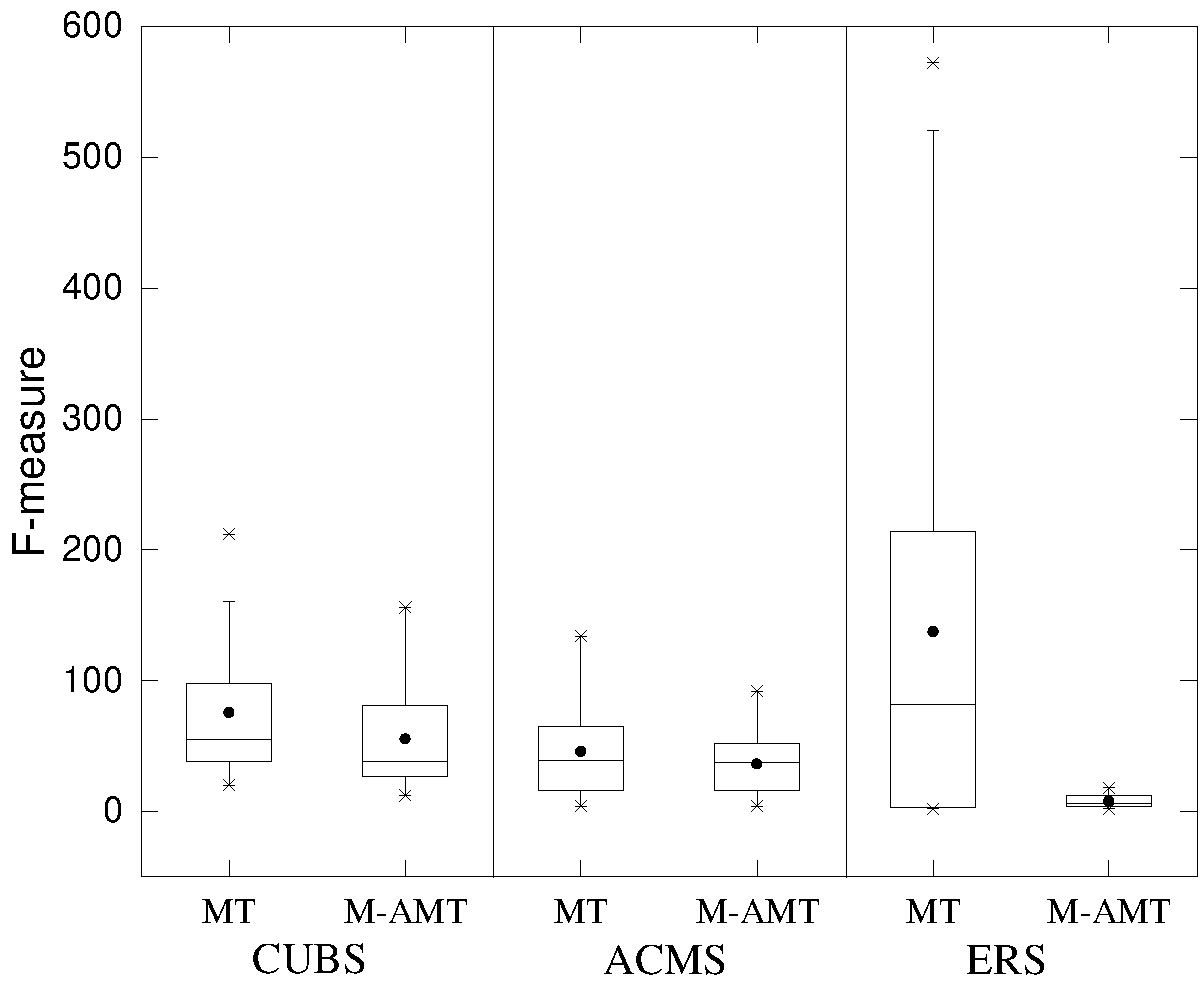
\includegraphics[width=0.5\textwidth]{figs//result//fmeasure}
  \caption{F-measure Boxplots for Each Program}
  \label{figure:fmeasure}
\end{figure}
\begin{figure}[!htp]
  \centering
  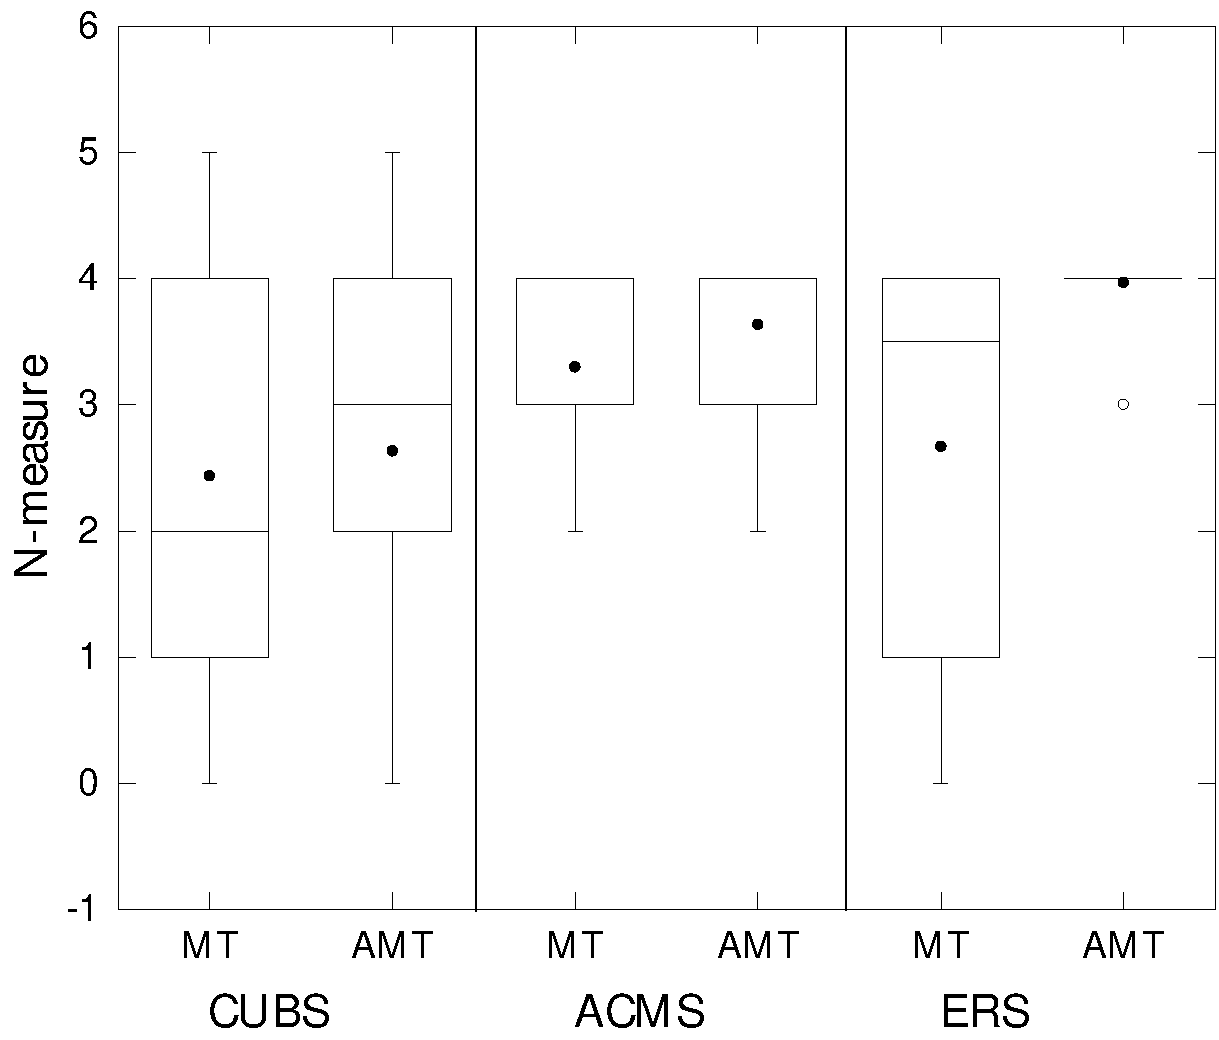
\includegraphics[width=0.5\textwidth]{figs//result//nmeasure}
  \caption{N-measure Boxplots for Each Program}
  \label{figure:nmeasure}
\end{figure}

\begin{table}
  \caption{F-measure and N-measure for studied programs}
  \label{table:results}
  \centering
  \begin{tabular}{|c|c|c|c|} \hline
    program                          &Strategy      &F-measure        &N-measure  \\ \hline
    \multirow{2}{*}{\texttt{CUBS}}   &MT            &75.60            &2.55       \\ \cline{2-4}
                                     &M-AMT         &55.30            &2.65       \\ \hline
    \multirow{2}{*}{\texttt{ACMS}}   &MT            &45.80            &3.45       \\ \cline{2-4}
                                     &M-AMT         &36.10            &3.20       \\ \hline
    \multirow{2}{*}{\texttt{ERS}}    &MT            &139.50           &2.80       \\ \cline{2-4}
                                     &M-AMT         &7.70             &3.95       \\ \hline
  \end{tabular}
\end{table}

From Table \ref{table:results} and Figures \ref{figure:fmeasure} and \ref{figure:nmeasure}, we have the following observations:
\begin{enumerate}[(1)]
  \item
  MT executes test cases in a random manner, that is, MT randomly selects test cases from input domain as source test cases, which does not use of any information returned from the
  testing process. Based on MT, M-AMT introduces software cybernetics \cite{cai2002optimal} into MT, analyzing the current test results to select ``better'' test cases that is more
  likely to detect faults.
  \item
  M-AMT need fewer test cases to detect the first fault for all three programs compared to the MT in terms of F-measure.
  \item
  Executing the same number of test cases, M-AMT reveals more faults than MT for all three programs.
\end{enumerate}

\subsubsection{RQ2: Selection Overhead}
\begin{table}
  \caption{F-time and N-time for studies programs (in ms)}
  \label{table:time}
  \centering
  \begin{tabular}{|c|c|c|c|} \hline
    program                          &Strategy      &F-time           &N-time  \\ \hline
    \multirow{2}{*}{\texttt{CUBS}}   &MT            &5.76             &10.24       \\ \cline{2-4}
                                     &M-AMT         &28.45            &71.70       \\ \hline
    \multirow{2}{*}{\texttt{ACMS}}   &MT            &3.79             &15.24       \\ \cline{2-4}
                                     &M-AMT         &28.85            &137.00       \\ \hline
    \multirow{2}{*}{\texttt{ERS}}    &MT            &29.05            &4.15       \\ \cline{2-4}
                                     &M-AMT         &4.10             &51.60       \\ \hline
  \end{tabular}
\end{table}

The detailed results of F-time and N-time are summarized in the Table \ref{table:time}, on the basis of which, we have the following observations:
\begin{enumerate}[(1)]
  \item
  \emph{the performance of the test techniques:} The traditional MT that randomly selects test cases and executes them. M-AMT first adjusts test profile according to current test
  results, then selects test cases and executes them. Our results indicate that MT selection test cases consumes less time than M-AMT.
  \item
  \emph{In terms of F-time and N-time:} In most of scenarios (except for F-time of ERS), MT selection test cases consumes less time than M-AMT. M-AMT require additional computation
  compared to MT and such additional computation is compensated by having fewer program executions. When the test case execution time saved by M-AMT is sufficient to cover the
  additional computation, M-AMT will have a better performance. To detect the first fault of ERS, M-AMT requires far fewer test cases than MT, hence M-AMT selection test cases
  consumes less time than MT.
\end{enumerate}

In summary, M-AMT outperformed tradition MT across F- and N-measure, which means that The fault detection efficiency of M-AMT is higher than MT. Meanwhile, M-AMT takes extra time to
adjust the test profile and select a partition, while such overhead can be compensated by having fewer programs executions.  This further indicates that between the proposed
M-AMT and traditional MT, M-AMT should be used.


\section{Related Work}
\label{section:related}
In this section, we describe related work from two perspectives: improvement on MT and improvement on RT and PT.

\subsection{Improvement on MT}
To alleviate the oracle problem, Chen et al. \cite{chen1998metamorphic} proposed a technique named metamorphic testing (MT) that has been receiving increasing attention
in the software testing community\cite{barr2015oracle, segura2016survey, chen2018metamorphic}. The main contributions to MT in the literature focused on the following
aspects: \rmnum{1}) MT theory; \rmnum{2}) combination with other techniques; \rmnum{3}) application of MT.
\begin{enumerate}[(1)]
  \item
  \emph{Theoretical development of MT:} The MRs and the source test cases are the most important components of MT. However, defining MRs can be difficult. Chen et al.
  \cite{chen2016metric} proposed a specification-based method and developed a tool called MR-GENerator for identifying MRs based on category-choice framework\cite{ostrand1988category}.
  Zhang et al. \cite{zhang2014search} proposed a search-based approach to automatic inference of polynomial MRs for a software under test, where a set of parameters is used to
  represent polynomial MRs, and the problem of inferring MRs is turn into a problem of searching for suitable values of the parameters. Then, particle swarm optimization is
  used to solve the search problem.
  Sun et al. \cite{sun2016mumt} proposes a data-mutation directed metamorphic relation acquisition methodology, in which data mutation is employed to construct input relations
  and the generic mapping rule associated with each mutation operator to construct output relations.
  Liu et al. \cite{liu2012new} proposed to systematically construct MRs based on some already identified MRs.

  Without doubt, ``good'' MRs can improve the fault detection efficiency of MT.
  Chen et al. \cite{chen2004case} reported that good MRs are those that can make the execution of the source-test case as different as possible to its follow-up test case.
  This perspective has been confirmed by the later studies \cite{dong2013security, batra2011efficient}.
  Asrafi et al. \cite{asrafi2011testing} conduct a case study to analyze the relationship between the execution behavior and the fault-detection effectiveness of metamorphic relations
   by code coverage criteria, and the results showed a strong correlation between the code coverage achieved by a metamorphic relation and its fault-detection effectiveness.

  Source test cases also have a important impact on the fault detection effectiveness of MT.
  Chen et al. \cite{chen2004metamorphic} compared the effects of source test cases generated by special value testing and random testing on the effectiveness of MT, and found that
   MT can be used as a complementary test method to special value testing.
  Batra and  Sengupta \cite{batra2011efficient} integrated genetic algorithms into MT to select source test cases maximising the the paths traversed in the software under test.
  Dong et al. \cite{dong2013security} proposed a Path--Combination--Based MT method that first generates symbolic input for each executable paths and minis relationships among these
  symbolic inputs and their outputs, then constructs MRs on the basis of these relationships, and generates actual test cases corresponding to the symbolic inputs.

  Different from the above investigates, we focused on performing test cases and MRs with fault revealing capabilities as quickly as possible by making use of feedback information.
  We first divided the input domain into disjoint partitions, and randomly selected an MR to generate follow-up test cases depended on source test case of related input partitions,
  then updated the test profile of input partitions according to the results of test execution. Next, a partition was selected according to updated test profile, and an MR was
  randomly selected from the set of MRs whose source test cases belong to selected partition.
  \item
  \emph{Combination with other techniques:} In order to improve the applicability and effectiveness of MT, it has been integrated into other techniques.
  Xie et al. \cite{xie2013metamorphic} combined the MT with the spectrum-based fault localization (SBFL), extend the application of SBFL to the common situations where test oracles
  do not exist.
  Dong et al. \cite{dong2010security} proposed a method for improving the efficiency of evolutionary testing (ET) by considering MR when fitness function is constructed.
  Liu et al. \cite{liu2014metamorphic} introduced MT into fault tolerance and proposed a theoretical framework of a new technique called Metamorphic Fault Tolerance (MFT), which can
  handle system failure without the need of oracles during failure detection. In MFT, the trustworthiness of a test case depends on the number of violations or satisfactions of
   metamorphic relations. The more relations are satisfied and the less relations are violated, the more trustable test case is.
  \item
  \emph{Application of MT:}
  MT has been successfully applied in a number of application domains, including web service \cite{sun2011metamorphic, sun2012metamorphic, segura2018metamorphic}, computer
  graphics \cite{Jameel2015Test}, embedded systems \cite{Jiang2013Testing}, compilers \cite{le2014compiler}.


\end{enumerate}

\subsection{Improvement on RT and PT}
Cai et al. introduced software cybernetics \cite{cai2002optimal} to software testing, and proposed Adaptive Testing (AT) \cite{Cai07, hu2005case, hu2009improved}, which takes
advantage of feedback information to control the execution process, has been shown that AT outperforms RT in terms of T-measure and increasing the number of faults, which means
that AT has higher efficiency and effectiveness than RT. However, AT may require a very long execution time in practice. To alleviate this,
Cai et al. \cite{cai2009random} proposed DRT, which uses testing information to dynamically adjust the test profile. There are several things that can impact on DRT��s test efficiency.
Yang et al. \cite{Yang2014} proposed A-DRT, which adjusts parameters during the testing process.
Li et al.~\cite{li2015approach} developed O-DRT, which has an objective function and a pre-defined parameter $f$. During the testing process, if the value of the objective function
is greater than $f$, the test profile is adjusted to a theoretically optimal one.
Lv et al. \cite{Lv2011} introduced two parameters for adjusting probability of different partitions, namely $\epsilon$ for adjusting probability of partitions where a test case
detects a fault and $\delta$ for adjusting probability of partitions where a test case does not detect a fault, and $\epsilon$ should be larger than $\delta$. Furthermore, they
provided the guidance of setting $\epsilon$ and $\delta$ by an interval of $\epsilon/\delta$.
Based on DRT, Sun et al. \cite{sun2018adaptive} proposed a new technique named adaptive partition testing to increase the adaptability of DRT itself, where the test profile and
the probability adjusting factors are dynamically updated. Furthermore, they develop two algorithms, Markov-chain based adaptive partition testing and reward-punishment based
adaptive partition testing, to implement the proposed approach.

\section{Conclusion}
\label{section:conclusion}
Metamorphic testing (MT) is a promising technique that alleviates the oracle problem. To improve the efficiency of MT, the most of researchers focused on generating and selecting
the ``better'' metamorphic relations (the execution results of the test cases are more likely to violate them), ignoring the impact of the source test cases.  Differently, based
on the partition testing, we proposed an adaptive metamorphic testing technique that aim to control the execution process of MT and make use of the feedback information, improving
the fault detection efficiency of MT. Furthermore, We implement the proposed technique in AMTesting, to the best of our knowledge. Empirical studies have been conducted to evaluate
the performance of M-AMT and MT using three real-life programs. It has been shown that M-AMT could use significantly fewer test cases to detect the first fault than tradition MT.
Moreover, Executing the same number of test cases, M-AMT detected more faults than traditional MT.

In our future work, we plan to conduct experiments on more real-life programs to further validate the effectiveness of M-AMT, and identify the limitations of our approach.

\section*{Acknowledgment}

This research is supported by the
the National Natural Science Foundation of China (Grant No. 61872039),
Beijing Natural Science Foundation (Grant No. 4162040),
the Aeronautical Science Foundation of China (Grant No. 2016ZD74004), and
the Fundamental Research Funds for the Central Universities (Grant No. FRF-GF-17-B29).

\newcommand{\BIBdecl}{\setlength{\itemsep}{0.2 em}}

\bibliographystyle{IEEEtran}
\bibliography{AMT}


\end{document}
